\chapter{Computational modeling of transcription factor-DNA interactions}

Researchers employ various experimental methods to study how transcription factors interact with DNA, identifying sequences or genomic regions that indicate TF specificity for particular DNA patterns. This data serves as the foundation for the computational modeling of TF-DNA interactions. Different models are available today, from simple and widely used \ac{PWMs} to advanced deep learning models. This chapter will cover different models and techniques used to create them, highlighting resources that store these models and explore their applications in research.

  \section{Transcription factor DNA binding models}

    \subsection{Position weight matrices (PWMs)}

    The most popular and widely used representation of TF-DNA interactions is the \ac{PWMs} (also called weight matrices or \ac{PSSMs}) ({Figure \ref{tf_dna_models}}) \cite{ambrosini2020insights,weirauch2013evaluation,stormo2015dna}. Several steps are followed when building a PWM.

    \begin{figure}
      \centering
      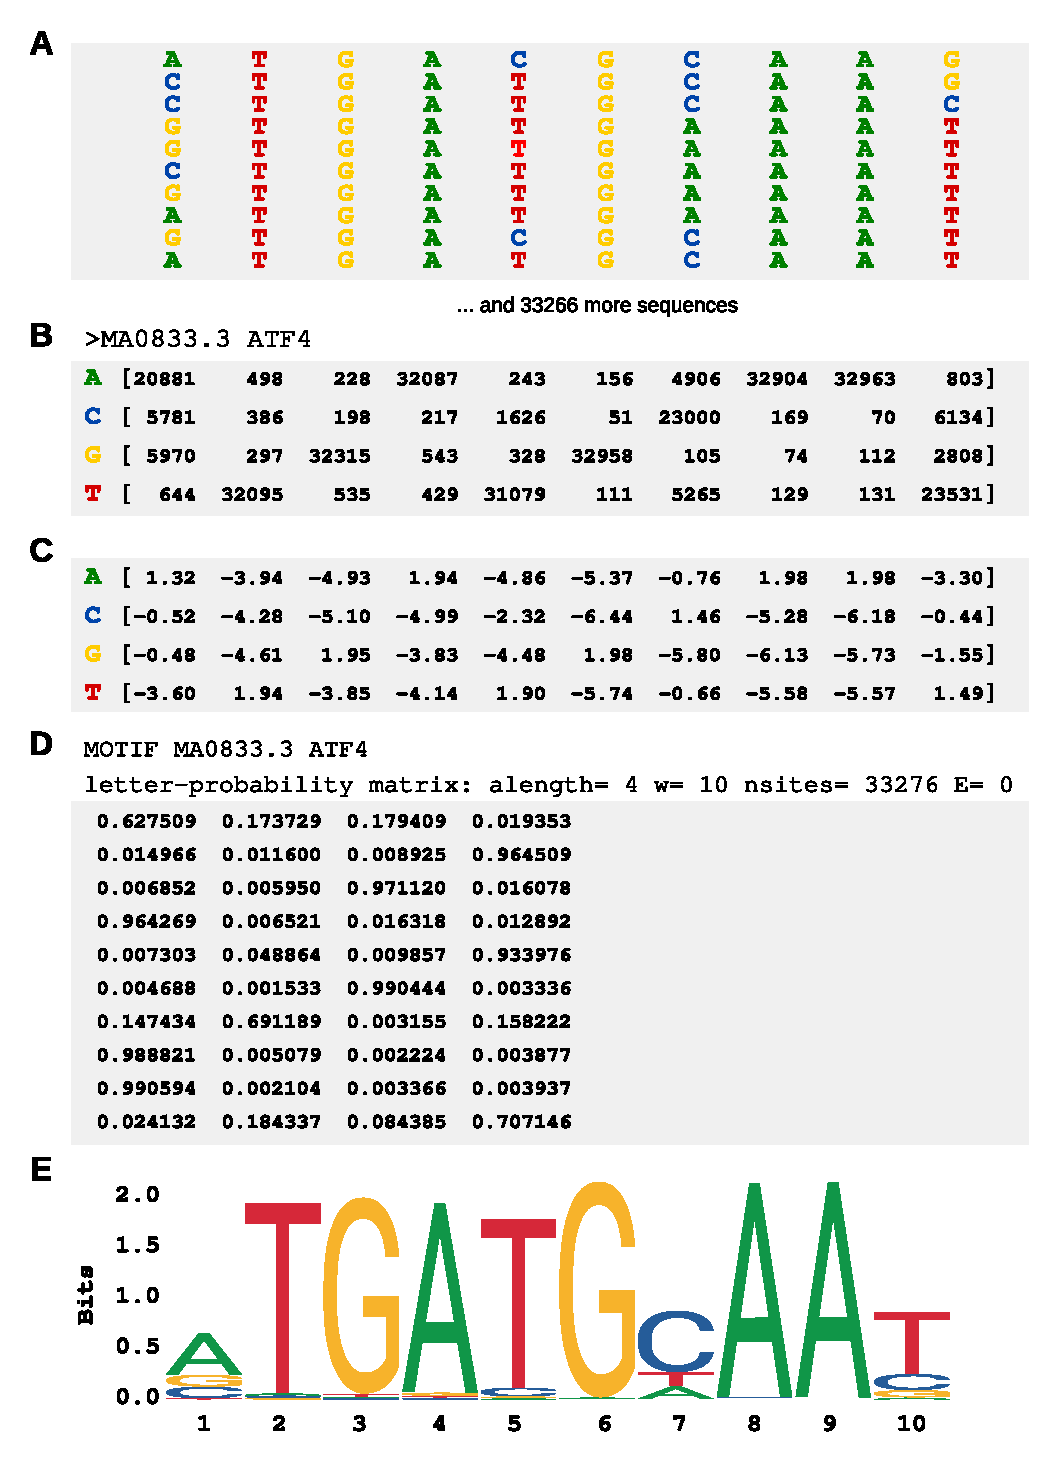
\includegraphics[scale=0.79]{figures/models/tf_dna_models.pdf}
      \caption[TF-DNA binding computational modelling]{\textbf{Modeling the binding of ATF4 transcription factor.} \textbf{A.} A set of aligned sequences bound by ATF4. Various experimental techniques can produce sequences. \textbf{B.} Position frequency matrix (PFM), which represents the nucleotide occurrence counts in each sequence position (visualized in JASPAR format). \textbf{C.} PFM can be converted into a position probability matrix (PPM) (visualized in MEME format). \textbf{D.} Position weight matrix (PWM) computed from the PPM. \textbf{E.} A sequence logo visualizes information content (IC) for the ATF4 binding profile. High values indicate a strong preference toward a particular base. Matrices from the JASPAR database ID MA0833.3.}
      \label{tf_dna_models}
    \end{figure}

    (1) From a set of aligned sequences (for example, processed experimental data or sequences collected from literature) that are bound by a TF of interest, a \ac{PFM} is computed ({Figure \ref{tf_dna_models}}A-B) \cite{ambrosini2018pwmscan}. A PFM, or a count matrix, is created by counting the occurrences of each nucleotide at each position \cite{stormo2013modeling,wasserman2004applied,weirauch2013evaluation}. The length of this matrix corresponds to the DNA motif length recognized by the TF \cite{ambrosini2020insights}. This matrix quantitatively describes the known \ac{TFBSs} \cite{wasserman2004applied}.

    (2) Counts can be converted into probabilities to build a \ac{PPM} ({Figure \ref{tf_dna_models}}C) using

    \begin{equation}
      p(b,i)=\frac{f_{b,i}+s(b)}{N+\sum\limits_{b'\in\{A,C,G,T\}}s(b')}
      \label{ppm}
    \end{equation}
    where $ p(b,i) $ is a probability of base $ b $ in position $ i $; $ f_{b,i} $ is counts of base $ b $ in position $ i $; $ s(b) $ is a pseudocount function; $ N $ is the number of sites. Pseudocounts can be added to each cell of the PFM to eliminate zeros \cite{wasserman2004applied}.

    (3) A PWM ({Figure \ref{tf_dna_models}}D) is constructed by dividing the nucleotide probabilities by expected background probabilities and converting the resulting values to a log scale (known and log odds ratio). The most straightforward model assumed equal 0.25 background probabilities for each base. The computation is done using

    \begin{equation}
      W_{b,i}=log_{2}\frac{p(b,i)}{p(b)}
      \label{pwm}
    \end{equation}
    where $ p(b) $ is the background probability of base $ b $; $ p(b,i) $ is the probability of base $ b $ in position $ i $; $ W_{b,i} $ is the PWM value or base $ b $ in position $ i $.

    Frequency or count matrices can be represented in multiple formats. For example, JASPAR format ({Figure \ref{tf_dna_models}}B) visualizes the counts, while MEME format visualizes the probabilities of each nucleotide in each position ({Figure \ref{tf_dna_models}}C). Some computational tools require specific format matrices, so familiarity with different count and probability representations is needed.

    It is difficult to interpret the actual DNA pattern preferentially bound by a TF only by looking at the PWM or PFM matrices. Therefore, sequence logos are used for visualization ({Figure \ref{tf_dna_models}}E). The sequence logo gives information about the frequency of each base at each position and the deviation from the expectation. Sequence logo visualizes \ac{IC} in bits. IC is a basic unit of information and quantifies how much information a binding site provides about the TF binding preferences. IC can be computed from probabilities using

    \begin{equation}
      D_{i}=2+\sum\limits_{b}p_{b,i}log_{2}p_{b,i}
      \label{ic}
    \end{equation}
    where $ D_{i} $ is the IC at position $ i $, $ p(b,i) $ is the probability of base $ b $ in position $ i $.

    All computational models used to model TF-DNA interactions are based on certain assumptions. One of the most significant limitations of PWMs is that these models assume the independence of nucleotides at different pairings \cite{wasserman2004applied,mathelier2013next,weirauch2013evaluation}. Locations of nucleotides at adjoining positions can be important for transcription factor binding, as was demonstrated through biochemical, statistical, and crystal structure analysis \cite{mathelier2013next}. Another potential caveat of the PWMs is their inability to accurately model compositional binding, as homodimers and heterodimers can have varying distances between the two binding sites \cite{wasserman2004applied,mathelier2013next}. The limitations of PWMs call for more complex models. One can expand the PWM model to capture additional information, such as DNA methylation \cite{grau2023widespread}. Other TF-DNA interaction models are described hereafter. However, despite their limitations, the availability and ease of use keep PFMs and PWMs the primary methods to model TF-DNA interactions.

    \subsection{Other more complex models}

    Other more complex models were introduced to address the limitations of PWMs. For example, the \ac{DWMs} extend the PWMs by considering pairs of adjacent nucleotides (dinucleotides) instead of individual nucleotides \cite{siddharthan2010dinucleotide}. DMWs were shown to be accurate representations of TF binding sites, performing well when predicting those TFBSs. However, a DMW will contain the same information as the PWM if positions are completely uncorrelated \cite{siddharthan2010dinucleotide}.

    In 2013, \ac{HMMs} based \ac{TFFMs} were introduced. They model both successive position interdependence within TFBSs and variable length motifs, which simple PWM models cannot achieve \cite{mathelier2013next}. It was demonstrated through protein binding array studies that dependencies are more substantial between the neighboring positions in the binding site compared to others \cite{zhao2012improved}. In first-order TFFMs, an HMM state represents each position within a TFBS. Each HMM state in the first order-TFFM is then decomposed into four states (one per nucleotide) to build a detailed TFFM \cite{mathelier2013next}. TFFMs are built using experimentally validated TF-DNA interaction sequences.

    Machine learning, deep learning, in particular, is the most state-of-the-art approach for TF-DNA interaction modeling. These approaches address critical limitations of the simpler TF-DNA binding models \cite{wang2022towards}. In a deep-learning framework predicting activity from a sequence, one-hot encoded DNA sequences are used as input ({Figure \ref{deep_learning_modeling}}A) \cite{novakovsky2023obtaining}. One needs to prepare training, validation (used for selecting methods, hyperparameter tuning, and avoiding overfitting), and testing datasets (used for model evaluation) \cite{koido2024fundamentals}. Different types of neural network architectures are built to train the deep learning models \cite{koido2024fundamentals}. For example, \ac{CNNs} have convolutional layers to detect the motifs, pooling layers to reduce the dimensionality, and fully connected layers to make predictions about TF binding affinity ({Figure \ref{deep_learning_modeling}}B) \cite{novakovsky2023obtaining}. The models are trained to classify binding vs. non-binding or predict the strength of the binding ({Figure \ref{deep_learning_modeling}}C). Finally, the model's predictive performance is evaluated. To describe the motifs and sequence features, the model needs to be interpreted by understanding the inner workings of the so-called "black box" models ({Figure \ref{deep_learning_modeling}}D) \cite{novakovsky2023obtaining}. For instance, one can derive PWMs from the first-layer neurons encoded in convolutional weight matrices. A more common strategy is to search for subsequences that activate a layer and then construct a PWM from aligned activating sequences \cite{novakovsky2023obtaining}. Interpretation of the models often requires additional tools based on certain assumptions, limiting deep learning-based approaches \cite{novakovsky2023obtaining}.

    \begin{figure}
      \centering
      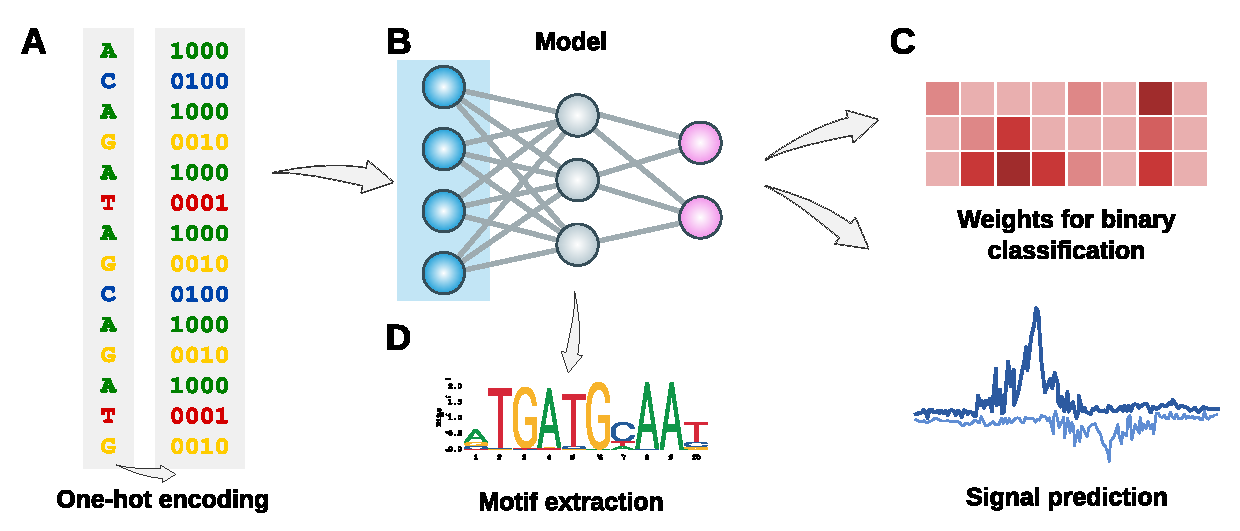
\includegraphics[width=1\textwidth]{figures/deep_learning/DL_models_latest.pdf}
      \caption[Deep learning approach to model TF-DNA interactions]{\textbf{Deep learning approach to model TF-DNA interactions.} \textbf{A}. DNA sequences are one-hot encoded before being used as input to the model. \textbf{B}. The neural network consists of multiple layers that make predictions. \textbf{C}. The model can predict the scores for epigenetic marks and the signal of TF binding. \textbf{D}. DNA binding motifs can be extracted from the network layers by interpreting the deep learning models.}
      \label{deep_learning_modeling}
    \end{figure}

    The pioneering approach created to detect motifs and predict TF binding sites is DeepBind \cite{alipanahi2015predicting}. Another method, DeepSea, was developed to predict multiple chromatin features in addition to the TF binding events \cite{zhou2015predicting,koido2024fundamentals}. The deep learning approaches are particularly relevant for deciphering and modeling cooperative TF binding. One of the latest approaches used to predict binding profiles of TFs and demonstrated cooperative action is BPNet \cite{avsec2021base}. BPNet is a CNN and models the TF binding at base resolution. It consists of multiple convolutional layers and predicts the TF binding signal in \ac{mESCs} for four TFs (Oct4, Sox2, Nanog, and Klf4). To interpret the results from the BPNet and retrieve the DNA motifs, another tool, TF-MoDISco, is required \cite{shrikumar2018technical}. The recurrent patterns are highlighted by aggregating the importance scores across aligned high-scoring regions in the sequences. Candidate consensus motifs are identified by clustering and aligning high-scoring sequence segments. Motifs are then filtered and scored based on their importance and prevalence. Finally, motifs can be visualized for more straightforward interpretation and annotated using collections of known motifs. In their study, the authors of BPNet demonstrated that their analyzed TFs are binding using soft syntax rules, which means there are no strict requirements on the numbers of nucleotides between the two TFs co-binding the region. The results also showed that Nanog binds with helical periodicity and TF cooperativity directionally \cite{avsec2021base}.

    \subsection{\textit{De novo} motif discovery}

    When analyzing TF-DNA interaction data, such as ChIP-seq, one can find over-represented sequence motifs using existing collections of DNA binding motifs (see the section on databases of TF-DNA binding models). However, motif collections are always limited, so to discover new motifs, \textit{de novo} motif discovery approaches have been developed \cite{boeva2016analysis}. \textit{De novo} motif discovery is a process inferring enriched DNA patterns in a set of DNA sequences compared to the background expectations \cite{stormo2013modeling}. The aim of \textit{de novo} motif discovery is to find short, statistically over-represented DNA patterns in the input set of sequences \cite{lihu2015review,das2007survey}. The used background can be a Markov model with nucleotide frequencies similar to the input or random sequences, such as shuffled original input sequences. Algorithms discover motifs in sequences derived from experimental methods, such as SELEX, \ac{PBM}, and ChIP-based techniques \cite{boeva2016analysis}.

    "Word-based" approaches gather approximate occurrences of a \textit{k}-mer in the input sequences and rank them based on their over-representation. RSAT \textit{peak-motifs} relies on several of such algorithms, namely oligo-, position-, and dyad-analysis ({Table \ref{de_novo_tools}}) \cite{,thomas2011rsat,thomas2012rsat,santana2022rsat}. Oligo-analysis detects over-represented oligonucleotides, while position-analysis identifies oligonucleotides with heterogeneous positional distributions in a provided set of sequences \cite{van1998extracting,helden2000statistical,thomas2011rsat}. By default, word-based analysis performs 6 and 7 bp length motif search \cite{thomas2012rsat}. Dyad-analysis detects spaced motifs, which dimeric TFs can bind \cite{helden2000discovering,thomas2011rsat}. Researchers observed that regulatory sites in the yeast genome often contain pairs of highly conserved trinucleotides, separated by non-conserved positions \cite{helden2000discovering}. RSAT \textit{peak-motifs} can also perform differential analysis (oligo-diff) when the control set is provided \cite{thomas2012rsat}.

    On the other hand, "profile-based" algorithms iteratively optimize an initial PWM and perform heuristic searches. These methods select positions from the input set, align the sequences, and then build and score the PWM \cite{lihu2015review}. For example, the computational tool MEME starts the motif search with multiple \textit{k}-mers, then it selects the current best to be optimized using \ac{EM} \cite{bailey1994fitting,zambelli2013motif}. One of the main limitations is that the presence of the motif is assumed in each input sequence \cite{lihu2015review}. STREME is the newest motif discovery tool from the authors of MEME that allows larger sets of input sequences ({Table \ref{de_novo_tools}}) \cite{bailey2021streme}.

    \begin{table}[htbp]
      \centering
      \caption[An overview of \textit{de novo} motif discovery tools]{\textbf{An overview of \textit{de novo} motif discovery tools.} Several computational tools are developed to find overrepresented sequence patterns.}
      \label{de_novo_tools}
      \begin{tabular}{p{0.175\linewidth} p{0.55\linewidth} p{0.14\linewidth}}
          \toprule
          \textbf{Tool}
          & 
          \textbf{Description}
          &
          \textbf{Reference}
          \\
          \midrule
          MEME
          & 
          Profile-based algorithm; uses expectation maximization (EM); finds recurring, fixed-length, ungapped patterns.
          &
          \cite{bailey1994fitting}
          \\[0.3ex]
          STREME
          &
          Profile-based algorithm; uses suffix tree-based optimization; finds recurring, fixed-length (3-30 bp), ungapped patterns.
          &
          \cite{bailey2021streme}
          \\[0.3ex]
          RSAT
          &
          Word-based algorithm; oligo-, position-, and dyad-analysis; finds variable size motifs.
          &
          \cite{thomas2011rsat,thomas2012rsat,santana2022rsat}
          \\
          \bottomrule
      \end{tabular}
  \end{table}

    All the above-mentioned computational tools have their strengths and weaknesses. For example, RSAT integrates a useful additional feature that compares discovered motifs with known motifs (read more about motif comparison in the section about the use of TF-DNA binding models). However, one of the main limitations is that these tools (except the RSAT dyad-analysis algorithm) aim to discover a single over-represented pattern in a set of sequences at a time. Specialized approaches would be needed to examine the relationship between different discovered patterns. The co-occurring patterns can indicate the TF cooperative binding.

    \subsection{Non-negative matrix factorization for motif discovery}

    A different approach from the above, \ac{NMF}, could be used for DNA pattern discovery in sequences. Matrix factorization (also referred to as matrix decomposition) is a class of unsupervised techniques that infers low-dimensional structure from high-dimensional data \cite{stein2018enter}. NMF is one of the matrix factorization techniques. All matrix factorization algorithms generally learn two matrices: pattern and amplitude \cite{stein2018enter}.

    Before applying NMF on genomic sequences, the usual practice is to one-hot encode the nucleotide sequences. It is a classical categorical data processing step for machine learning approaches. Each nucleotide is assigned a unique four-bit long code ({Figure \ref{nmf_motif_discovery}}A). Individual sequences are converted into a numerical array, which then can be passed to the NMF algorithm ({Figure \ref{nmf_motif_discovery}}B). A number of patterns that the NMF needs to learn is a hyperparameter and needs to be pre-defined. The learned pattern matrix represents the relationships between the nucleotides \cite{stein2018enter}. Each row in the pattern matrix contains the contribution weight of each nucleotide at each position in the pattern. The amplitude matrix describes relationships between the sequences\cite{stein2018enter}. Each column in the amplitude matrix stores continuous weights that describe the relative contribution of each sequence in each inferred pattern. Each pattern gets a set of sequences assigned with the highest contribution scores. The two matrices can be used to distinguish subsets of sequences with particular patterns that can be represented as DNA sequence motifs. NMF has a hyperparameter $ k $, instructing how many patterns should be learned. For example, with $ k = 4 $, four DNA patterns are learned from an input set of DNA sequences ({Figure \ref{nmf_motif_discovery}}C).

    NMF is the basis of a computational tool, seqArchR, to identify position-specific DNA patterns in promoter regions and decipher promoter architectures \cite{nikumbh2023identifying}. It is known that specific DNA motifs inform the selection of TSSs and are located at fixed distances from them. The seqArchR package can identify TSS-directing and lineage-specific motifs, such as TATA or nucleosome position signals. Defining combinations of these motifs can be used to classify promoter architectures and associate them with specific gene regulatory programs \cite{nikumbh2023identifying}.

    A limitation of NMF for motif discovery is that the algorithm takes arrays as the input, meaning the input genomic sequences must be the same length. Another significant limitation is that sequence patterns that NMF can distinguish have to occur at fixed distances. Various patterns can be discovered in separate patterns, but there must be enough sequences with the same pattern at the exact location. Lastly, a hyperparameter $ k $ can be challenging to define. While several methods have been introduced to estimate the cophenetic correlation coefficient to determine the number of patterns, there is no convergence on an optimal method \cite{brunet2004metagenes}.

    \begin{figure}
      \centering
      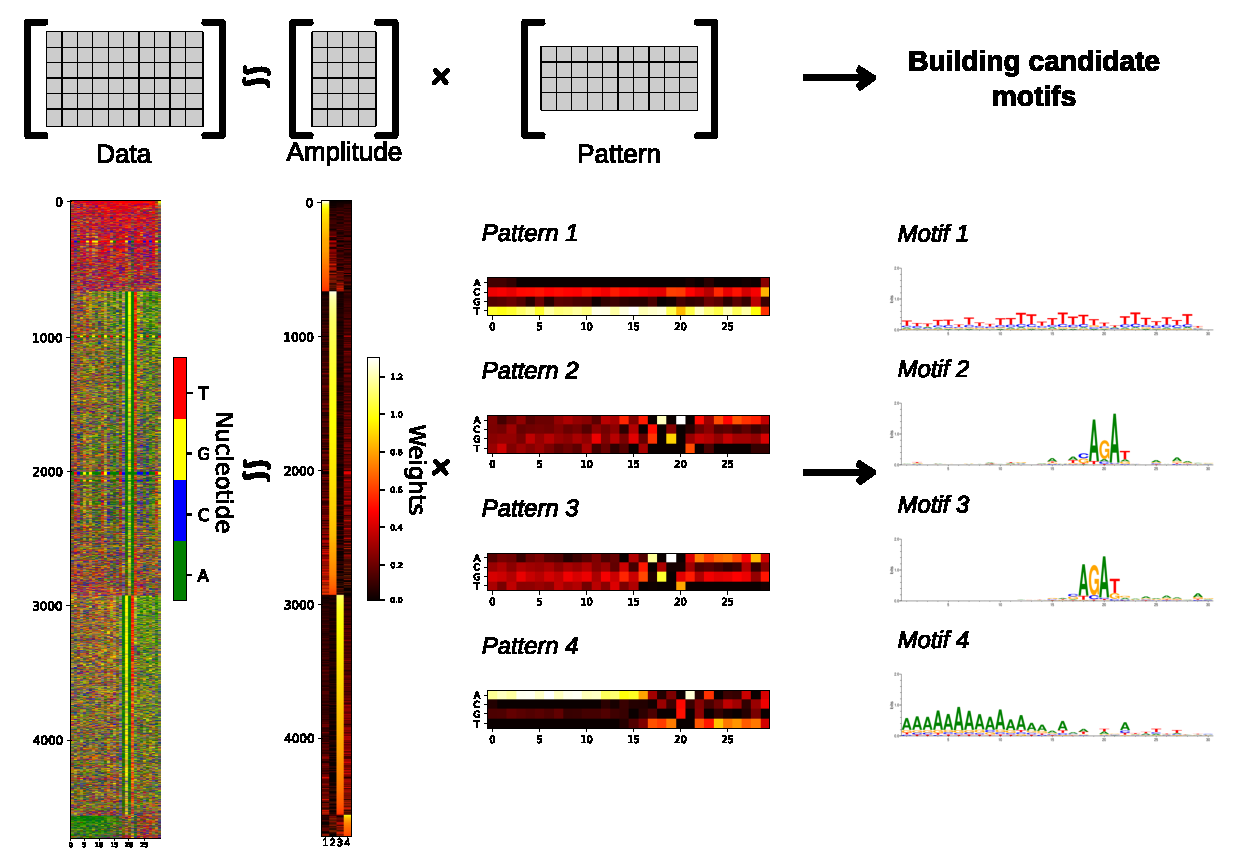
\includegraphics[width=1\textwidth]{figures/nmf/nmf_for_discovery_latest.pdf}
      \caption[NMF for DNA pattern discovery]{\textbf{Application of non-negative matrix factorization for DNA pattern discovery in sequences.} An example of 4 patterns NMF applied to a set of one-hot encoded DNA sequences (data matrix). The data matrix is factorized into amplitude and pattern matrices. Candidate DNA patterns (motifs) can be built using the resulting matrices. Each pattern produces one motif. Adapted from \cite{rauluseviciute2023identification}.}
      \label{nmf_motif_discovery}
    \end{figure}

  \section{Databases of TF-DNA interaction models}

  Several repositories store PWMs. For example, JASPAR, TRANSFAC, HOCOMOCO, and CIS-BP ({Table \ref{motif_databases}}) \cite{rauluseviciute2024jaspar,matys2006transfac,wingender2008transfac,vorontsov2024hocomoco,weirauch2014determination}. For the users of such resources, it is essential to understand what data is stored and how it is retrieved and processed. JASPAR is an open-access database and stores DNA binding motifs for TFs from six taxa. All motifs in JASPAR are manually curated. JASPAR discovers motifs from experimental data, such as ChIP-seq or DAP-seq, or mined as PFMs from various resources (for instance, a selection of CIS-BP database motifs) and publications. Independent evidence found by curators supports CORE collection motifs. In addition to motif collections, JASPAR provides analyzed data, such as motif clusters and various tools \cite{rauluseviciute2024jaspar}. TRANSFAC also stores curated DNA motifs with experimentally determined and predicted binding sites. However, the complete database is not open-access \cite{matys2006transfac,wingender2008transfac}. HOCOMOCO is a publicly available resource that compiles and stores human and mouse TF binding motifs. The motifs in the latest release of the database are human-curated and automatically benchmarked \cite{vorontsov2024hocomoco}. Finally, CIS-BP is also open-access and contains motifs for more than a thousand TFs from 131 diverse eukaryotes. Motifs are generated using \ac{PBM}, SELEX, or ChIP-seq data but are also mined from other motif resources, such as TRANSFAC and JASPAR. A unique feature of CIS-BP is that the database offers inferred motifs. Based on the similarity of the DBDs, two TFs are binding similar motifs. Therefore, it is possible to assume a binding profile from one TF to a closely related other TF \cite{weirauch2014determination}.

  \begin{table}[htbp]
    \centering
    \caption[An overview of motif databases]{\textbf{An overview of DNA binding motif databases.}}
    \label{motif_databases}
    \begin{tabular}{p{0.175\linewidth} p{0.55\linewidth} p{0.14\linewidth}}
        \toprule
        \textbf{Database}
        & 
        \textbf{Content}
        &
        \textbf{Reference}
        \\
        \midrule
        JASPAR
        & 
        Open-access manually curated collections of DNA binding motifs for six taxonomic groups. The CORE collection contains motifs with orthogonal support.
        &
        \cite{rauluseviciute2024jaspar}
        \\[0.3ex]
        TRANSFAC
        &
        Curated collection of TF binding motifs.
        &
        \cite{wingender2008transfac}
        \\[0.3ex]
        HOCOMOCO
        &
        Open-access manually curated motif collections of human and mouse TFs.
        &
        \cite{vorontsov2024hocomoco}
        \\[0.3ex]
        CIS-BP
        &
        Open-access database with a comprehensive list of predicted TFs from >300 species. Motifs are available if known.
        &
        \cite{lambert2018human}
        \\
        \bottomrule
    \end{tabular}
\end{table}

  Even if current databases contain thousands of motifs from various species, it is essential to keep these resources updated by adding new data and refining the old. Finally, new ways of TF-DNA modeling (such as deep-learning models) motivate the expansion or creation of new databases that could offer a variety of TF-DNA interaction models to the community.

  \section{Use of position weight matrices}

  Researchers use the collections of known TF binding profiles in numerous ways. One of the most critical applications is the prediction of TF binding sites. Computational tools predict putative TFBSs in the entire genome or perform TF binding enrichment in a set of regions. Another popular application of the TF motifs is an annotation of \textit{de novo} discovered motifs, which is needed when no binding preferences are known for a TF of interest.

    \subsection{Prediction of TF binding sites}

    TF-DNA binding models can be used to predict putative transcription factor binding sites in the entire genome (also referred to as motif scanning) or a set of regions of interest (for example, ChIP-seq peaks or promoters) \cite{boeva2016analysis}. The TF binding models for predicting can be taken from various databases overviewed in the previous section \cite{rauluseviciute2024jaspar,matys2006transfac,wingender2008transfac}.

    In TFBS prediction, algorithms first score sequences using a PWM. The sliding window approach is used to scan a DNA sequence of interest. Each window (same size as a PWM) is scored. When scoring, the weights of each corresponding nucleotide in a PWM are summed to estimate the TF binding probability in a given DNA sequence using

    \begin{equation}
      S=\sum\limits_{i=1}^{w}W_{l_{i},i}
      \label{scoring}
    \end{equation}
    where $ S $ is a score for input sequence; $ w $ is the width of the PWM; $ l_{i} $ is the position $ i $ in the input sequence \cite{wasserman2004applied}.
    The final set of TFBS predictions is separated from the background and defined after applying the score threshold. Usually, statistical significance (measured through \textit{p}-value) is evaluated to solve the thresholding issue. For example, it can be the computation of the probability to observe at least the same number of motif instances with a specific cutoff in a random sequence with total length (equal to the total size of sequences in the set of regions of interest) \cite{boeva2016analysis}. This task becomes difficult computationally if one tries to score multiple motifs (possibly with overlaps), which is relevant when investigating TF cooperativity and co-binding.

    The prediction tool will find fewer motif instances with the higher score cutoff, and the resulting binding sites will likely correspond to the strong binding affinity. Compared with the lower cutoff, the algorithm predicts more sites, and they might represent both strong and weak binding sites \cite{boeva2016analysis}. However, the "futility theorem" states that predicted TFBSs outnumber the sites that are actually occupied by a TF \cite{wasserman2004applied}. False positively predicted TFBSs are not available for binding due to chromatin structure or local epigenetic properties \cite{mathelier2013next}.

    Resources, such as JASPAR, in addition to the collections of PFMs, offer TFBS predictions for the most popular genome assemblies \cite{rauluseviciute2024jaspar}. Bioinformaticians designed various tools that scan or find over-represented motifs in regions. For example, PWMScan, FIMO, or HOMER \cite{weidemuller2021transcription,grant2011fimo,heinz2010simple}.

    \subsection{Prediction of direct TF binding sites}

    According to the "futility theorem", only a subset of predicted TFBSs are occupied by a TF. Identifying those TFBSs can be challenging. One way to address this and provide TFBSs with stronger confidence is to combine experimental data with computational models, such as PWMs. This strategy is employed to compute TFBSs stored in the UniBind database ({Figure \ref{unibind}}) \cite{puig2021unibind,gheorghe2019map}.

    \begin{figure}
      \centering
      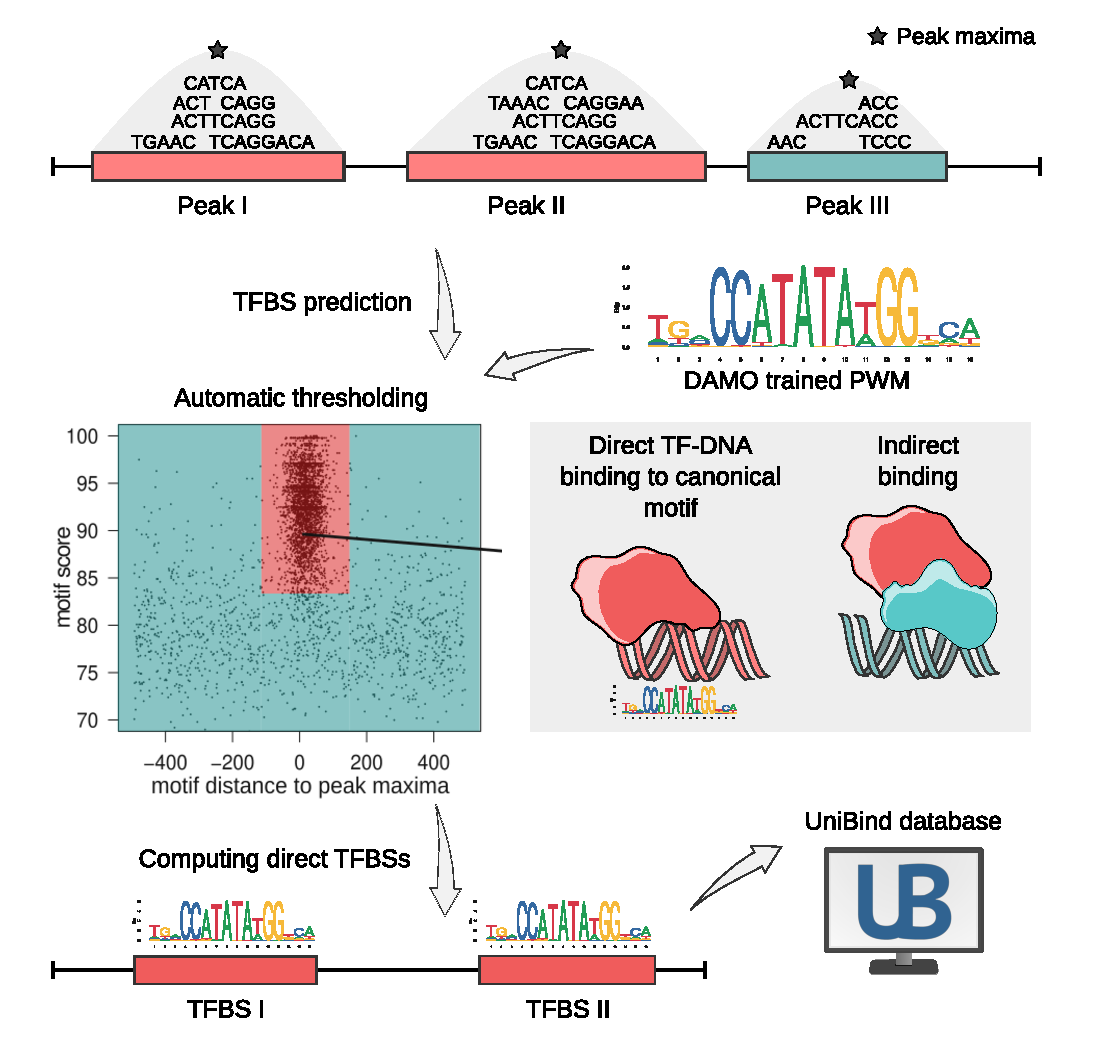
\includegraphics[width=0.9\textwidth]{figures/unibind/unibind_latest.pdf}
      \caption[Use of TF-DNA binding models to infer direct TF-DNA interactions]{\textbf{An example of combining experimental data with computational models to infer direct TF-DNA interactions.} The ChIP-eat pipeline takes ChIP-seq data in peaks and predicts transcription factor binding sites (TFBSs) using the DAMO-trained position weight matrix (PWM) of the profiled TF. The automatic thresholding selects TFBSs, which represent direct TF-DNA binding to the canonical motif (red), from the rest of the predictions, representing indirect or unspecific binding (blue). The final sets of direct TFBSs are collected for each analyzed dataset and compiled into the UniBind database. Adapted from \cite{puig2021unibind}.}
      \label{unibind}
    \end{figure}

    Current experimental techniques aim to identify TF binding, but in practice, the data reflect direct and indirect or non-specific TF binding \cite{furey2012chip}. It is challenging to separate the two signals computationally. In addition, while the TFs interact with the DNA through short motifs, the ChIP-seq peaks are usually hundreds of base pairs long. A peak summit defines a location within the peak where the signal (the amount of ChIP-seq reads) is the highest. The ChIP-eat computational approach identifies TFBSs that the TF of interest directly binds. The method combines ChIP-seq peak data and PWMs to produce sets of direct TFBSs ({Figure \ref{unibind}}) \cite{puig2021unibind,gheorghe2019map}. Given a set of peaks and a PWM, the TFBS enrichment zone is detected using an automatic threshold. The enrichment zone contains TFBSs with high PWM scores and close proximity to ChIP-seq peak summits. The resulting set of TFBSs represent direct TF-DNA interactions \cite{puig2021unibind,gheorghe2019map}. The resulting TFBSs are of the size of the DNA binding motif. TFBSs from 9 species are provided to the community as a UniBind database \cite{puig2021unibind}. UniBind TFBSs can be a great starting point for further analysis. For example, enrichment analysis can identify enriched TFBSs in a set of regions of interest and provide information on the transcription regulation driving TFs \cite{puig2021unibind}.

    \subsection{Annotating \textit{de novo} discovered motifs}

    Another use of collections of TF binding profiles is an annotation of \textit{de novo} discovered motifs. Computational tools are designed to compare the motifs of interest against the provided collection of known motifs. For example, TOMTOM compares the query motif against a database of target motifs. It allows for gapped motif-motif alignments, computes the p-value for each motif, and performs a Bonferroni correction to derive motif E value. TOMTOM integrates a variety of metrics to score similarity (for example, Euclidian distance and Pearson's correlation) \cite{gupta2007quantifying}. RSAT also has a tool, \textit{compare-matrices}, to annotate discovered motifs when the known motif library is provided \cite{thomas2011rsat,santana2022rsat}. The tool can compare two collections of PWMs, and TOMTOM uses different similarity scoring functions. Multiple or all metrics can be compared and later summarized by computing the mean rank \cite{thomas2011rsat}.

    \subsection{Prediction of TF co-binding events}

    As with \textit{de novo} motif discovery, predicting TF binding sites is usually limited to individually analyzing each TF binding profile, so deciphering the possible co-occurrence of TF motifs requires specialized tools. The prediction of a co-binding event usually focuses on the prediction of a secondary motif near known TFBSs (primary motif), which could indicate a potential binding of a cooperating TF ({Figure \ref{predicting_cobinding}}). Out of all sequences with a primary motif, a subset might not have any co-binding events ({Figure \ref{predicting_cobinding}}A), have a predicted secondary motif with a specific spacer and orientation from the primary motif ({Figure \ref{predicting_cobinding}}B) or have more than one predictions with specific spacings ({Figure \ref{predicting_cobinding}}C). Prediction of the secondary motif is as important as determining the motif grammar.
    
    SpaMo is a computational tool that analyzes co-binding events using a library of known motifs to detect possible co-binding TFs relative to the indicated primary TF \cite{whitington2011inferring}. The method was developed to analyze ChIP-seq data, where the profiled TF is the primary TF. It summarizes the spacing and orientation between the primary and secondary motifs and provides information on the match's significance. The algorithm tests every secondary motif to determine whether the predicted TFBSs have enriched spacing concerning the primary TFBSs \cite{whitington2011inferring}. A significant limitation of SpaMo and similar tools is the requirement of known TF binding motif libraries, meaning previously uncharacterized DNA patterns are missed.

    \begin{figure}
      \centering
      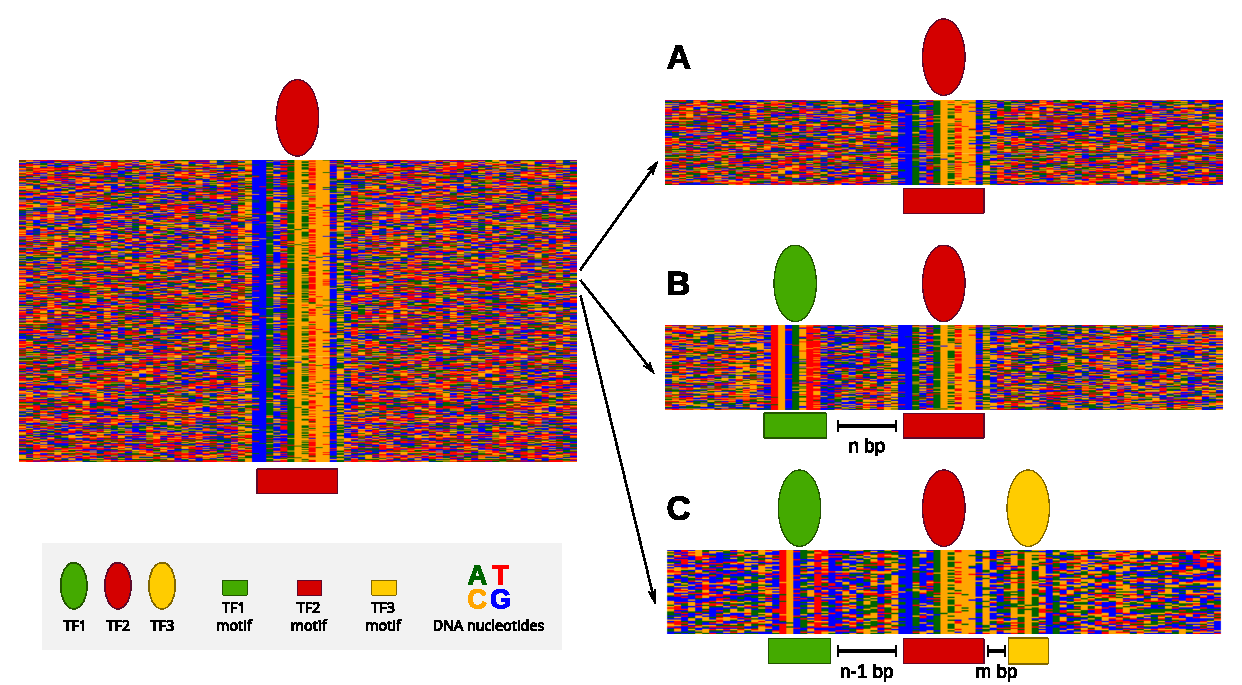
\includegraphics[width=1\textwidth]{figures/cooperation_problem/cooperation_problem_latest.pdf}
      \caption[Prediction of TF co-binding events]{\textbf{Prediction of TF co-binding events.} Co-binding events can be investigated by discovering co-binding motifs. A set of genomic sequences with known TFBSs harbor a primary motif bound by a TF2. Some of these sequences do not contain any secondary motif that could indicate a potential co-binding event (\textbf{A}). Other sequences can harbor a secondary motif n bp upstream of the primary and potentially bound by a TF1 (\textbf{B}) or two motifs: TF1 motif a shorter distance from the primary and TF3 that is m bp downstream of the primary motif (\textbf{C}).}
      \label{predicting_cobinding}
    \end{figure}

    It is crucial to consider the context in which individual TFs are binding. The cooperative binding of multiple TFs in the regulatory regions enables fine-tuning transcription. Therefore, developing computational tools for analyzing such mechanisms would be beneficial in expanding our knowledge about TF cooperativity.
